\documentclass{article}

% ── NeurIPS 2026 style ────────────────────────────────────────────────────────
% Pass natbib options before NeurIPS loads it
\PassOptionsToPackage{numbers,sort&compress}{natbib}
% "preprint" shows author names and adds "Preprint" footer (appropriate for
% course projects that are not blind submissions)
\usepackage[preprint]{neurips_2026}

% ── Packages ──────────────────────────────────────────────────────────────────
\usepackage[utf8]{inputenc}
\usepackage[T1]{fontenc}
\usepackage{amsmath,amssymb,amsfonts}
\usepackage{nicefrac}
\usepackage{booktabs}
\usepackage{multirow}
\usepackage{graphicx}
\usepackage{subcaption}
\usepackage{xcolor}
\usepackage{url}
\usepackage{hyperref}
\usepackage{cleveref}
\usepackage{enumitem}
\usepackage{array}

\hypersetup{
  colorlinks=true, linkcolor=blue!70!black,
  citecolor=blue!70!black, urlcolor=magenta!80!black
}

\newcolumntype{C}[1]{>{\centering\arraybackslash}p{#1}}
\newcolumntype{L}[1]{>{\raggedright\arraybackslash}p{#1}}

% ── Title ─────────────────────────────────────────────────────────────────────
\title{Semantic Similarity Measurement in Latent Space\\
       for LLM Prediction Evaluation}

\author{%
  Haodong Xu, Chi Kit WONG, Sida Zhang \\
  The Hong Kong University of Science and Technology (Guangzhou) \\
  AIAA 4051 --- Final Research Project Report
}

\begin{document}
\maketitle

% ── Abstract ──────────────────────────────────────────────────────────────────
\begin{abstract}
Evaluating Large Language Model (LLM) predictions remains challenging, particularly
in the presence of diverse valid answers and hallucinations.
This paper investigates whether cosine similarity in embedding space can serve as a
reliable proxy for factual correctness across four benchmark datasets spanning
short-form QA (SciQ, SimpleQA) and long-form QA (Natural Questions, TruthfulQA).
Using Qwen3-4B under both direct-answer (\emph{no-thinking}) and chain-of-thought
(\emph{thinking}) modes, we encode predictions and ground-truth answers with three
pretrained embedding models (BGE-base-en-v1.5, all-MiniLM-L6-v2, E5-base-v2) and
measure AUC as the primary discriminability metric.
Our main findings are: (1) cosine similarity is a strong correctness indicator for
short-form QA (AUC up to 0.976) but degrades substantially for long-form QA
(TruthfulQA AUC~0.72--0.81); (2) chain-of-thought reasoning hurts discriminability
for short answers but unexpectedly improves it for TruthfulQA; (3) E5-base-v2 is the
most robust embedding model across tasks.
We further conduct failure analysis, categorising errors into three types---lexical
variation, semantic ambiguity, and long-form reasoning complexity---and propose four
improvement methods. A trained hyperbolic projection (HELM-style) shows promising
held-out gains on TruthfulQA (+0.052--+0.098 AUC points), although direct comparison
with full-set post-hoc methods should be interpreted carefully because it is evaluated
on a held-out split.
Sentence-level MaxSim and span extraction provide complementary improvements in the
thinking mode.
Finally, compatibility experiments on the TA baseline artifacts confirm the
short-vs-long similarity gap after correcting the HHEM loading issue, with HHEM
providing discriminative labels for SciQ and TruthfulQA.
\end{abstract}

% ── 1. Introduction ───────────────────────────────────────────────────────────
\section{Introduction}
\label{sec:intro}

Large Language Models (LLMs) have achieved remarkable performance on a wide array of
question-answering (QA) benchmarks.
However, assessing the \emph{correctness} of generated responses at scale is itself a
non-trivial problem: exact-match metrics miss semantically equivalent paraphrases,
while task-specific rule sets are difficult to generalise.
An appealing alternative is to measure the \emph{semantic similarity} between a model
prediction and the ground-truth answer in a shared embedding space, using cosine
similarity as a lightweight, model-agnostic proxy for correctness.

This approach raises two fundamental questions.
First, is embedding similarity genuinely discriminative between correct and incorrect
predictions---and to what degree?
Second, does the answer depend on the \emph{type} of QA task (concise factual answers
vs.\ open-ended explanations)?

We address both questions with a controlled study spanning four datasets and three
embedding models, and extend the analysis with an ablation on LLM generation mode
(chain-of-thought reasoning vs.\ direct answers).
Our contributions are:
\begin{itemize}[nosep]
  \item A systematic benchmark comparing cosine-similarity discriminability across
        2 short-form and 2 long-form QA datasets (\Cref{sec:results});
  \item An ablation study on the effect of chain-of-thought reasoning on embedding
        similarity (\Cref{sec:ablation});
  \item A categorised failure analysis that attributes errors to lexical variation,
        semantic ambiguity, and long-form reasoning complexity
        (\Cref{sec:failure});
  \item Evaluation of four improvement strategies, including a trained hyperbolic
        projection that achieves consistent gains on TruthfulQA
        (\Cref{sec:improvement});
  \item A compatibility check against the TA baseline pipeline and full-size TA
        datasets, including an analysis of the original HHEM and MPNet artifacts
        (\Cref{sec:ta-baseline}).
\end{itemize}

% ── 2. Related Work ───────────────────────────────────────────────────────────
\section{Related Work}
\label{sec:related}

\paragraph{Embedding-based evaluation metrics.}
BERTScore~\citep{zhang2019bertscore} uses contextual token-level similarities from
BERT to evaluate text generation.
Sentence-BERT~\citep{reimers2019sentencebert} produces fixed-size sentence vectors
well-suited for semantic textual similarity (STS) benchmarks.
More recently, E5~\citep{wang2022text} and BGE~\citep{xiao2023cpack} establish
state-of-the-art results on MTEB~\citep{muennighoff2022mteb}, providing powerful
general-purpose embeddings.
However, none of these studies directly benchmark embedding similarity as a
\emph{correctness classifier} on diverse QA tasks.

\paragraph{Hallucination in LLMs.}
\citet{maynez2020faithfulness} and \citet{ji2023survey} characterise hallucination
as generation of plausible but factually unsupported content.
RAGTruth~\citep{wu2023ragtruth} provides a corpus of RAG hallucinations, revealing
that cosine similarity alone conflates faithful and unfaithful responses.
Our work explores this limitation systematically on non-RAG QA.

\paragraph{Chain-of-thought prompting.}
\citet{wei2022chain} showed that chain-of-thought (CoT) prompting substantially
improves multi-step reasoning.
Recent work has also noted that CoT can introduce verbose, off-topic text for smaller
models~\citep{kojima2022large}, potentially distorting embedding representations.
We test this hypothesis empirically using Qwen3-4B.

\paragraph{Hyperbolic embeddings for NLP.}
Poincar\'{e} embeddings~\citep{nickel2017poincare} and HELM~\citep{he2025helm}
demonstrate that hyperbolic geometry captures hierarchical semantic structure more
faithfully than Euclidean cosine similarity.
We evaluate a HELM-inspired trained projection head as an improvement strategy.

\paragraph{Summary.}
\Cref{tab:related} contrasts prior evaluation approaches and highlights the
limitations our work addresses.

% \begin{table}[t]
% \centering
% \caption{Comparison between prior evaluation methods and our study.}
% \label{tab:related}
% \begin{tabular}{p{0.20\linewidth} p{0.30\linewidth} p{0.38\linewidth}}
% \toprule
% \textbf{Method family} & \textbf{Representative work} & \textbf{Limitation addressed by our work} \\
% \midrule
% Lexical metrics & EM, token-F1 & Fail on paraphrases and semantic equivalence. \\
% Embedding metrics & BERTScore, SBERT, E5, BGE & Measure similarity, but not calibrated as correctness classifiers across diverse QA tasks. \\
% Factuality / NLI metrics & NLI-style consistency, HHEM & More factual but model-dependent and expensive. \\
% LLM-as-judge & GPT-style evaluators & Powerful but costly and less reproducible. \\
% Hyperbolic methods & Poincaré embeddings, HELM & Capture hierarchy, but require training rather than post-hoc mapping. \\
% \bottomrule
% \end{tabular}
% \end{table}

\begin{table}[t]
\centering
\caption{Comparison between prior evaluation methods and our study.}
\label{tab:related}
\small
\setlength{\tabcolsep}{4pt}
\renewcommand{\arraystretch}{1.08}
\begin{tabular}{@{}L{0.22\linewidth} L{0.24\linewidth} L{0.47\linewidth}@{}}
\toprule
\textbf{Method family} &
\textbf{Representative work} &
\textbf{Limitation addressed by our work} \\
\midrule
Lexical metrics &
EM, token-F1 &
Fail on paraphrases and semantic equivalence. \\

Embedding metrics &
BERTScore, SBERT, E5, BGE &
Measure similarity, but are not calibrated as correctness classifiers across diverse QA tasks. \\

Factuality / NLI metrics &
NLI-style consistency, HHEM &
More factual but model-dependent and expensive. \\

LLM-as-judge &
GPT-style evaluators &
Powerful but costly and less reproducible. \\

Hyperbolic methods &
Poincaré embeddings, HELM &
Capture hierarchy, but require training rather than post-hoc mapping. \\
\bottomrule
\end{tabular}
\end{table}

% ── 3. Methodology ────────────────────────────────────────────────────────────
\section{Methodology}
\label{sec:method}

% \begin{figure}[t]
%   \centering
%   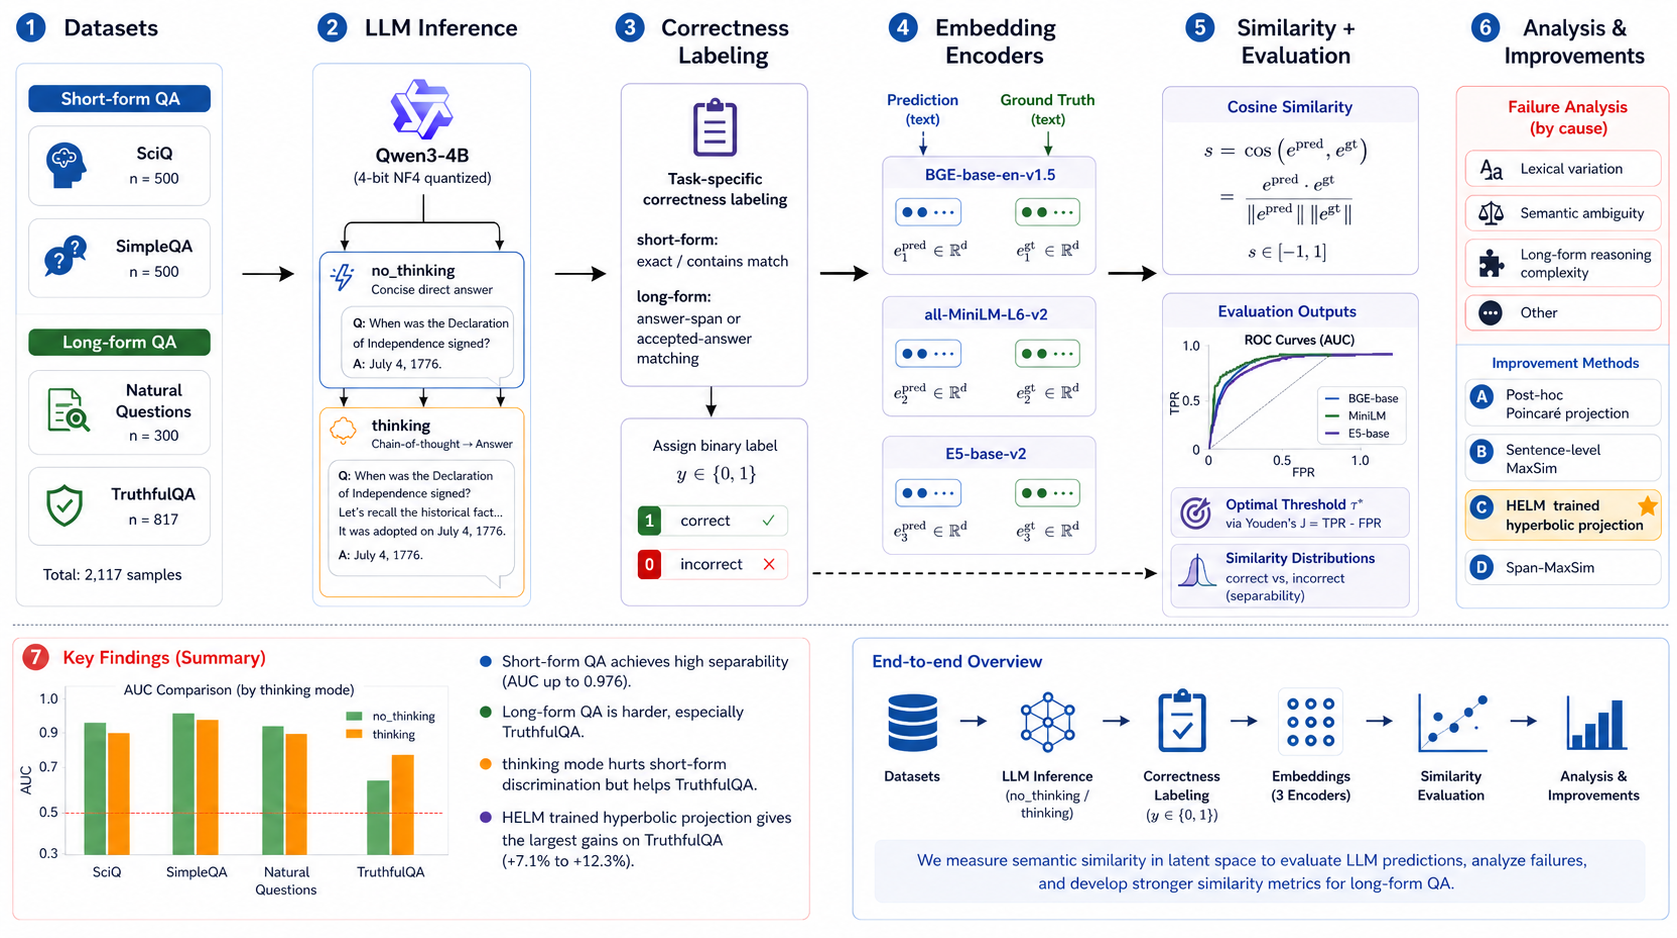
\includegraphics[width=\textwidth]{figures/method_figure_v1.png}
%   \vspace{-0.5em}
%   \caption{Overview of the proposed evaluation pipeline. The figure summarizes the
%   full process from dataset selection and LLM inference to correctness labeling,
%   embedding-based similarity scoring, AUC evaluation, failure analysis, and metric
%   improvement.}
%   \label{fig:method}
% \end{figure}

\begin{figure}[t]
  \centering
  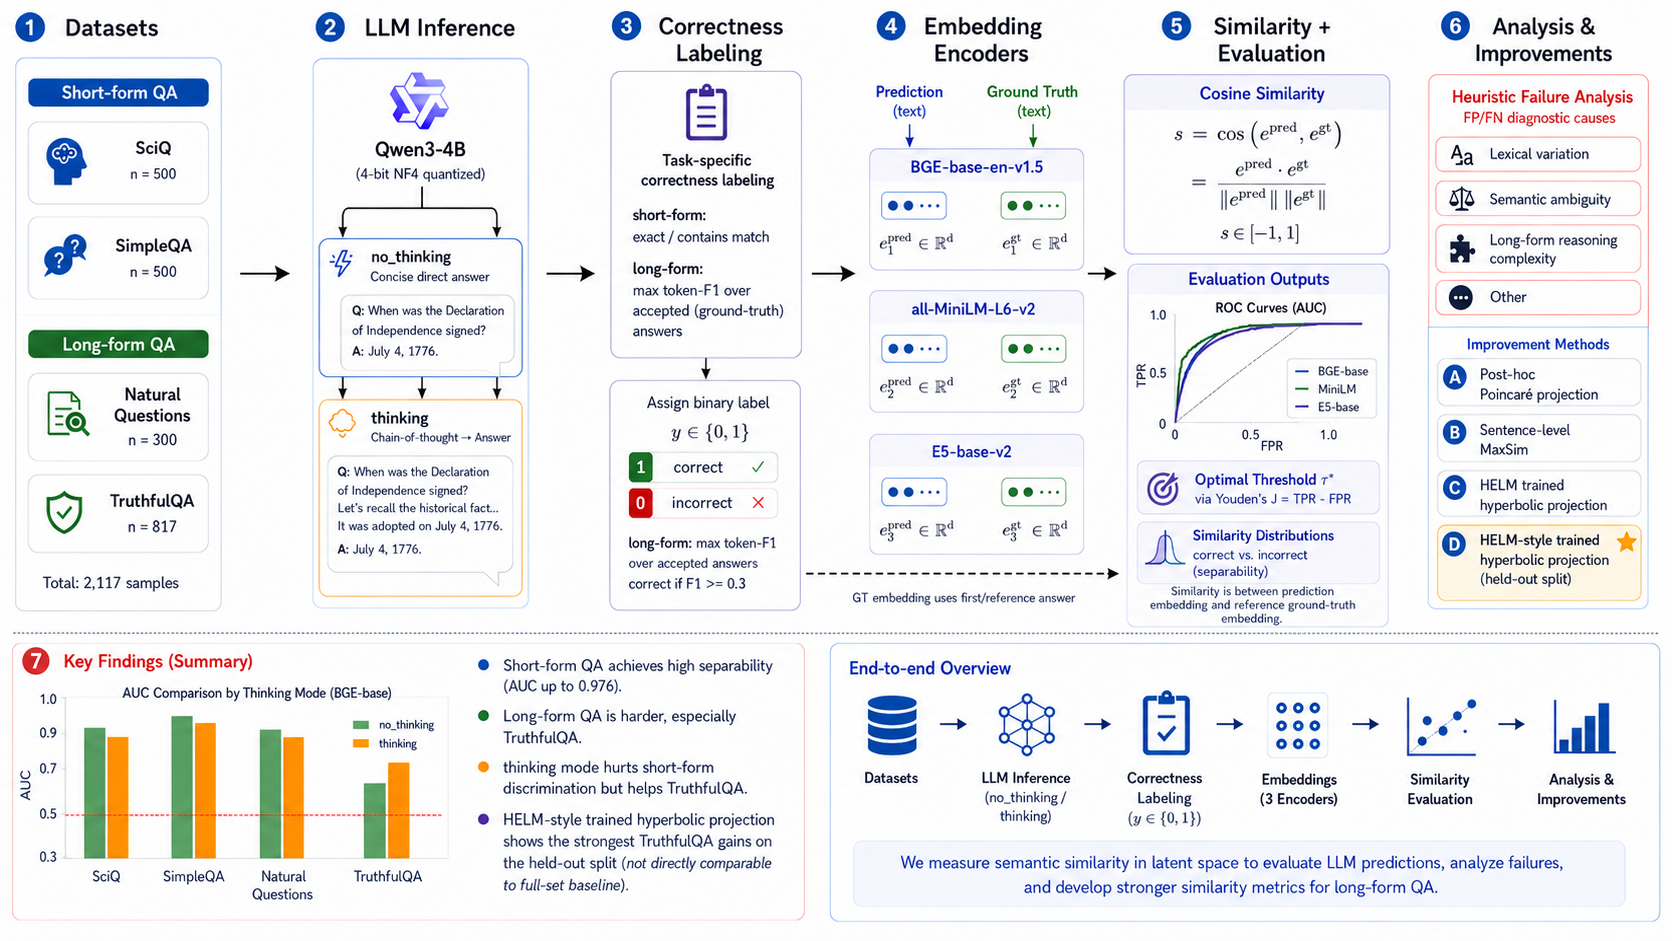
\includegraphics[width=\textwidth]{figures/method_figure_v2.png}
  \vspace{-0.5em}
  \caption{Overview of the proposed evaluation pipeline.}
  \label{fig:method}
\end{figure}

\Cref{fig:method} provides an end-to-end overview of our evaluation pipeline, including dataset construction, LLM inference, correctness labeling, embedding-based similarity scoring, downstream evaluation, failure analysis, and improvement methods.

\subsection{Datasets}

We evaluate on four publicly available datasets covering complementary QA regimes:

\begin{itemize}[nosep]
  \item \textbf{SciQ}~\citep{welbl2017sciq}: multiple-choice science questions with
        unambiguous, short ground-truth answers.  We sample 500 instances.
  \item \textbf{SimpleQA}~\citep{openai2024simpleqa}: single-hop factual questions
        with a single short answer string.  We sample 500 instances.
  \item \textbf{Natural Questions (NQ)}~\citep{kwiatkowski2019nq}: open-domain
        questions with short answer spans extracted from Wikipedia.
        We sample 300 instances.
  \item \textbf{TruthfulQA}~\citep{lin2021truthfulqa}: adversarially curated
        questions targeting common human misconceptions, with multiple valid
        answers.  All 817 instances are used.
\end{itemize}

\subsection{LLM Inference}

All predictions are generated by \textbf{Qwen3-4B}~\citep{qwen3} loaded at 4-bit
NF4 quantisation on a single NVIDIA GPU.
We run each dataset under two modes:

\begin{description}[nosep]
  \item[\texttt{no\_thinking}] Direct answer generation with temperature 0.
        Responses are typically one short sentence or phrase.
  \item[\texttt{thinking}] Chain-of-thought reasoning enabled via system prompt.
        Responses contain explicit reasoning steps before a final answer.
\end{description}

Correctness labels are produced by dataset-specific automatic rules.
For short-form datasets (SciQ and SimpleQA), we use normalized exact match with
substring-containment fallback:
\begin{equation}
  \text{is\_correct} = \max_i \bigl[\texttt{em}(p, g_i) + \texttt{contains}(p, g_i)\bigr] > 0
\end{equation}
where $p$ is the prediction and $\{g_i\}$ is the set of accepted answers.
For long-form datasets (NQ), we compute the maximum token-level F1 between the
prediction and the accepted ground-truth answers, and label a prediction as correct
when the score exceeds the configured threshold.
For TruthfulQA, the prediction is compared against the list of accepted correct answers.
These automatic labels serve as silver labels for evaluating embedding-score discriminability.

\subsection{Embedding Models}

Three pretrained sentence encoders are compared:
\begin{itemize}[nosep]
  \item \textbf{BGE-base-en-v1.5} (BAAI, 768-dim, 109M params)
  \item \textbf{all-MiniLM-L6-v2} (Sentence-Transformers, 384-dim, 22M params)
  \item \textbf{E5-base-v2} (Microsoft, 768-dim, 109M params)
\end{itemize}

\subsection{Similarity Computation and Evaluation}

Each prediction and each ground truth string are independently encoded.
The similarity score for a sample is:
\begin{equation}
  s = \frac{\mathbf{e}_p \cdot \mathbf{e}_g}{\|\mathbf{e}_p\|\,\|\mathbf{e}_g\|}
\end{equation}
where $\mathbf{e}_p$ and $\mathbf{e}_g$ are the $\ell_2$-normalised embeddings of
the prediction and (first) ground-truth answer, respectively.

Discriminability is measured by the \textbf{Area Under the ROC Curve (AUC)}.
A threshold $\tau^*$ is selected by maximising Youden's J statistic.
Statistical significance is assessed by two-sample $t$-tests comparing correct vs.\
incorrect similarity distributions.

% ── 4. Experimental Setup ─────────────────────────────────────────────────────
\section{Experimental Setup}
\label{sec:setup}

\paragraph{Correctness rate.}
The datasets exhibit different natural difficulty for Qwen3-4B
(\Cref{tab:accuracy}): SciQ is easiest (52--61\%), while SimpleQA is hardest (3.2\%).

\begin{table}[t]
\centering
\caption{Qwen3-4B correctness rate under the dataset-specific automatic labeling rule.}
\label{tab:accuracy}
\begin{tabular}{lrrrr}
\toprule
\textbf{Dataset} & \textbf{Type} & \textbf{no\_thinking} & \textbf{thinking} & $n$ \\
\midrule
SciQ       & Short & 52.2\% (261/500)  & 60.8\% (304/500) & 500 \\
SimpleQA   & Short &  3.2\% (16/500)   &  3.2\% (16/500)  & 500 \\
NQ         & Long  &  9.3\% (28/300)   &  4.0\% (12/300)  & 300 \\
TruthfulQA & Long  & 35.0\% (286/817)  & 28.2\% (230/817) & 817 \\
\bottomrule
\end{tabular}
\end{table}

\paragraph{Statistical validation.}
All 24 (dataset, mode, model) configurations yield $p \ll 0.001$ in
two-sample $t$-tests, confirming that the cosine similarity distributions of
correct and incorrect predictions are reliably separated (\Cref{tab:stats}).

\begin{table}[t]
\centering
\caption{Cosine similarity statistics (BGE, no\_thinking). All $p$-values $\ll 0.001$.}
\label{tab:stats}
\begin{tabular}{lrrrr}
\toprule
\textbf{Dataset} & $\bar{s}_{\text{correct}}$ & $\bar{s}_{\text{incorrect}}$ &
  $\Delta\bar{s}$ & $p$-value \\
\midrule
SciQ       & 0.921 & 0.693 & \textbf{+0.228} & $3.96\times10^{-84}$ \\
SimpleQA   & 0.925 & 0.554 & \textbf{+0.371} & $5.94\times10^{-10}$ \\
NQ         & 0.742 & 0.516 & +0.226          & $1.23\times10^{-11}$ \\
TruthfulQA & 0.791 & 0.678 & +0.113          & $1.45\times10^{-22}$ \\
\bottomrule
\end{tabular}
\end{table}

% ── 5. Results and Analysis ───────────────────────────────────────────────────
\section{Results and Analysis}
\label{sec:results}

\subsection{Main Results}

\Cref{tab:main} reports AUC across all 24 configurations.
The corresponding ROC curves for BGE-base are shown in \Cref{fig:roc}.

\begin{table}[t]
\centering
\caption{AUC (Area Under ROC Curve) for all dataset / mode / embedding-model combinations.
Best per dataset/mode in \textbf{bold}.}
\label{tab:main}
\setlength{\tabcolsep}{5pt}
\begin{tabular}{ll ccc ccc}
\toprule
\multirow{2}{*}{\textbf{Dataset}} & \multirow{2}{*}{\textbf{Type}}
  & \multicolumn{3}{c}{\textbf{no\_thinking}}
  & \multicolumn{3}{c}{\textbf{thinking}} \\
\cmidrule(lr){3-5}\cmidrule(lr){6-8}
  & & BGE & MiniLM & E5 & BGE & MiniLM & E5 \\
\midrule
SciQ       & Short & 0.940 & \textbf{0.954} & 0.933 & 0.902 & 0.934 & 0.890 \\
SimpleQA   & Short & \textbf{0.976} & 0.933 & 0.931 & 0.934 & 0.879 & 0.886 \\
NQ         & Long  & 0.905 & 0.894 & \textbf{0.934} & 0.880 & 0.869 & \textbf{0.899} \\
TruthfulQA & Long  & 0.743 & 0.723 & 0.784 & 0.801 & 0.763 & \textbf{0.813} \\
\bottomrule
\end{tabular}
\end{table}

Key observations:
\begin{itemize}[nosep]
  \item Short-form AUC is uniformly high (0.879--0.976), confirming that cosine
        similarity is a reliable correctness proxy for concise factual answers.
  \item TruthfulQA exhibits markedly lower AUC (0.72--0.81), reflecting the
        difficulty of separating correct from plausible-but-wrong answers in
        adversarial long-form settings.
  \item E5-base-v2 is the most robust model: it ranks first or second in 5 of 8
        (dataset, mode) combinations and achieves the best cross-task average AUC.
\end{itemize}

\begin{figure}[t]
  \centering
  \begin{subfigure}[b]{0.48\textwidth}
    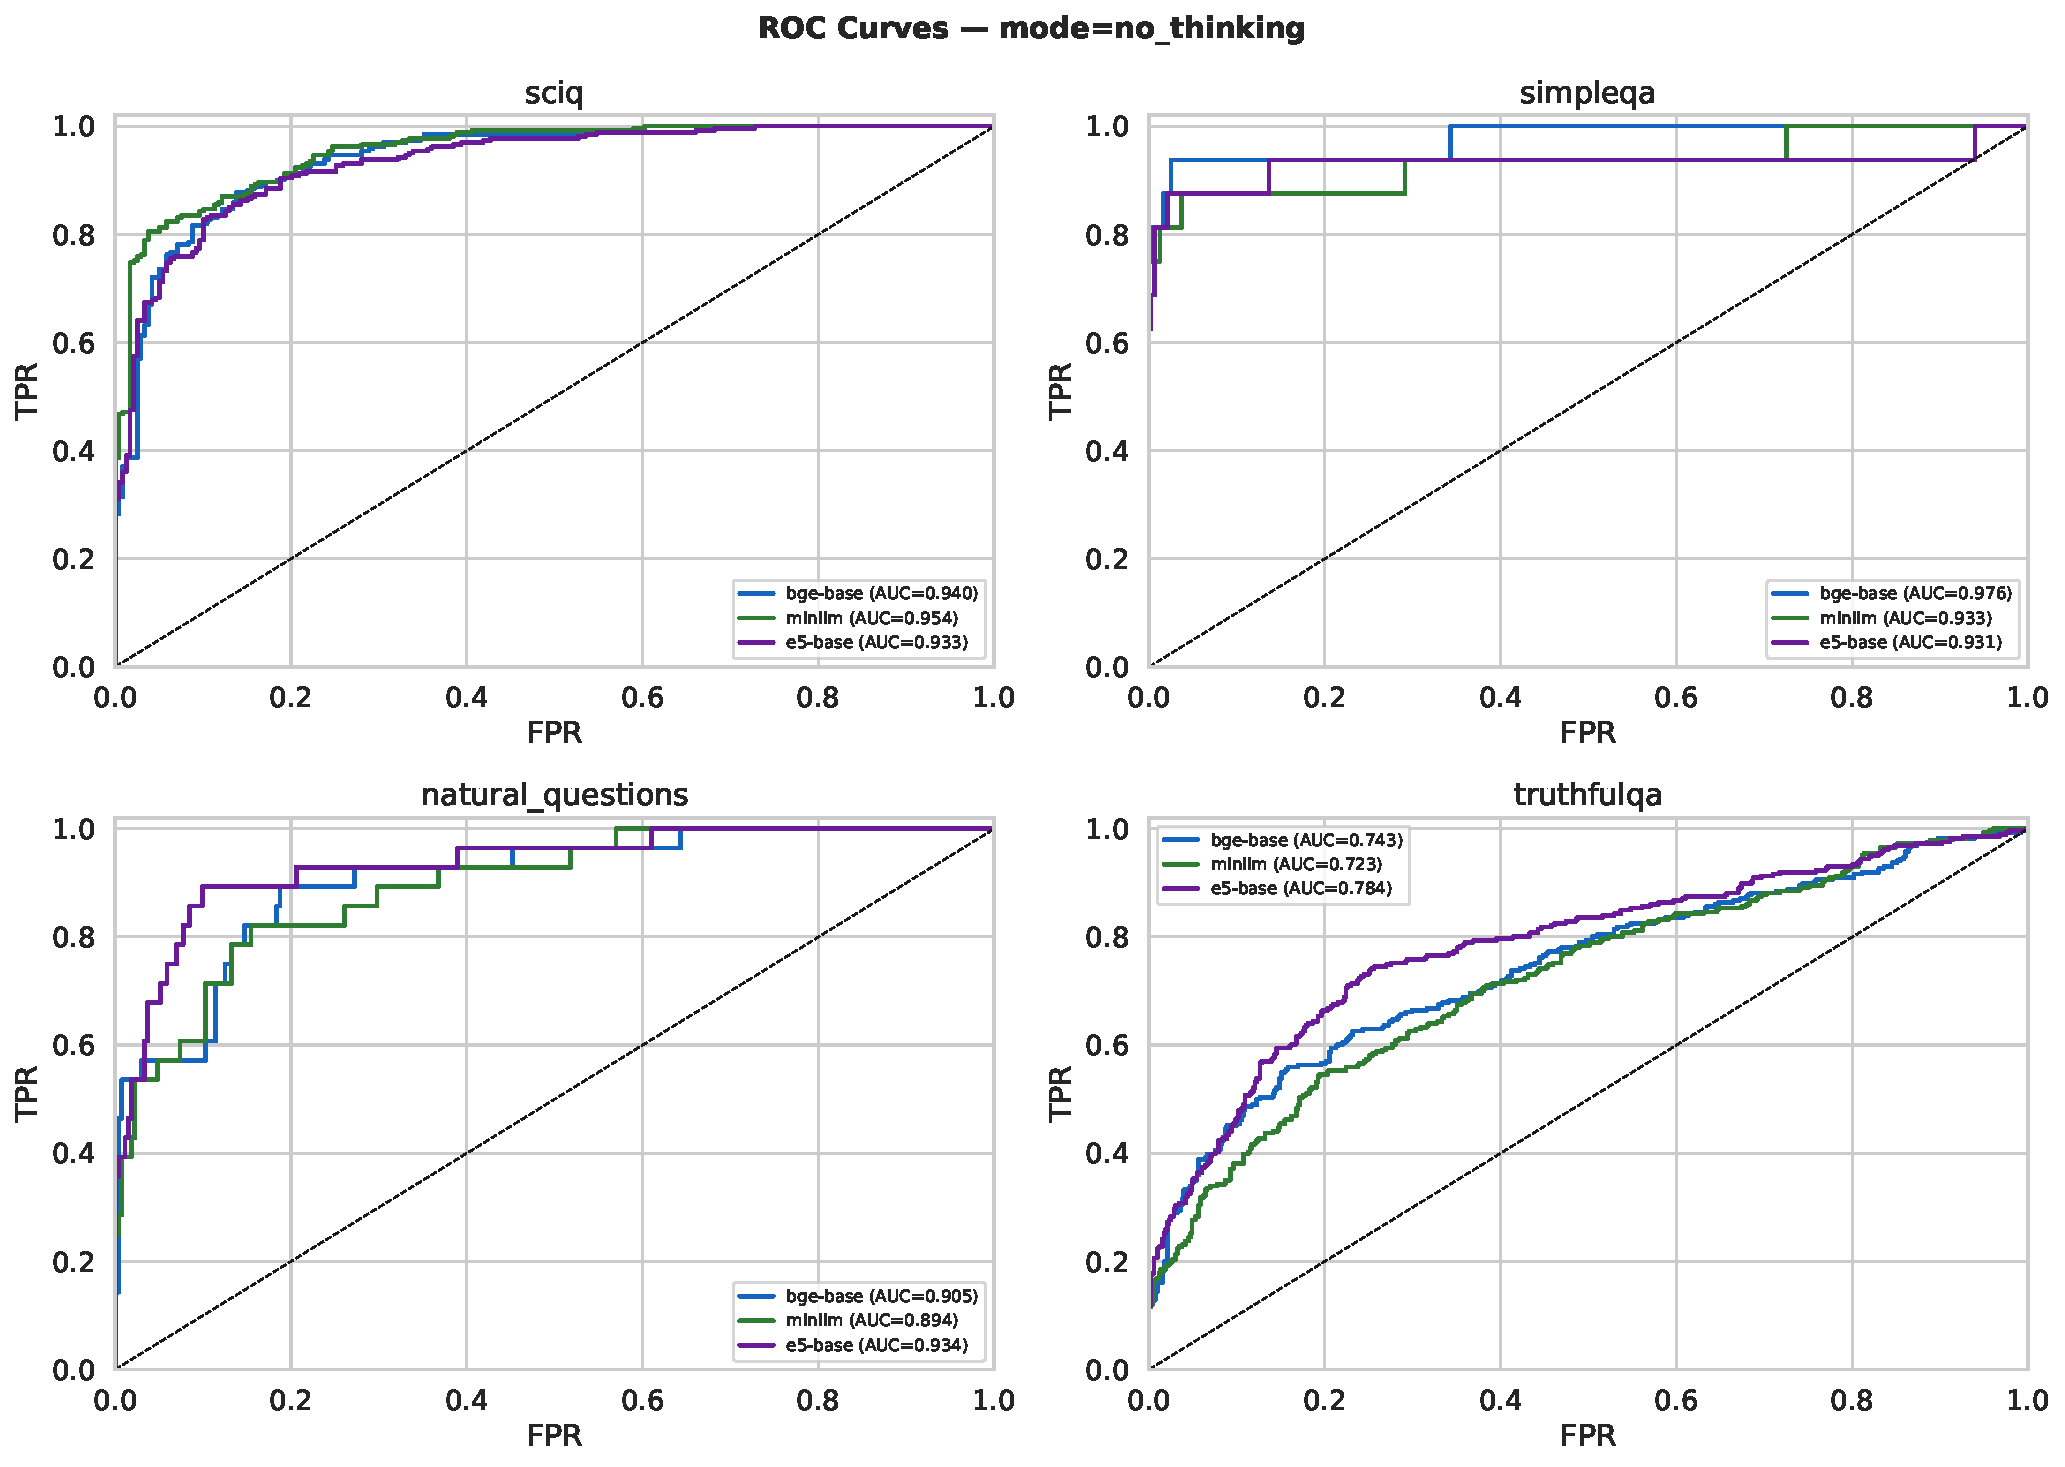
\includegraphics[width=\linewidth]{figures/roc_no_thinking.pdf}
    \caption{ROC curves --- no\_thinking mode}
  \end{subfigure}\hfill
  \begin{subfigure}[b]{0.48\textwidth}
    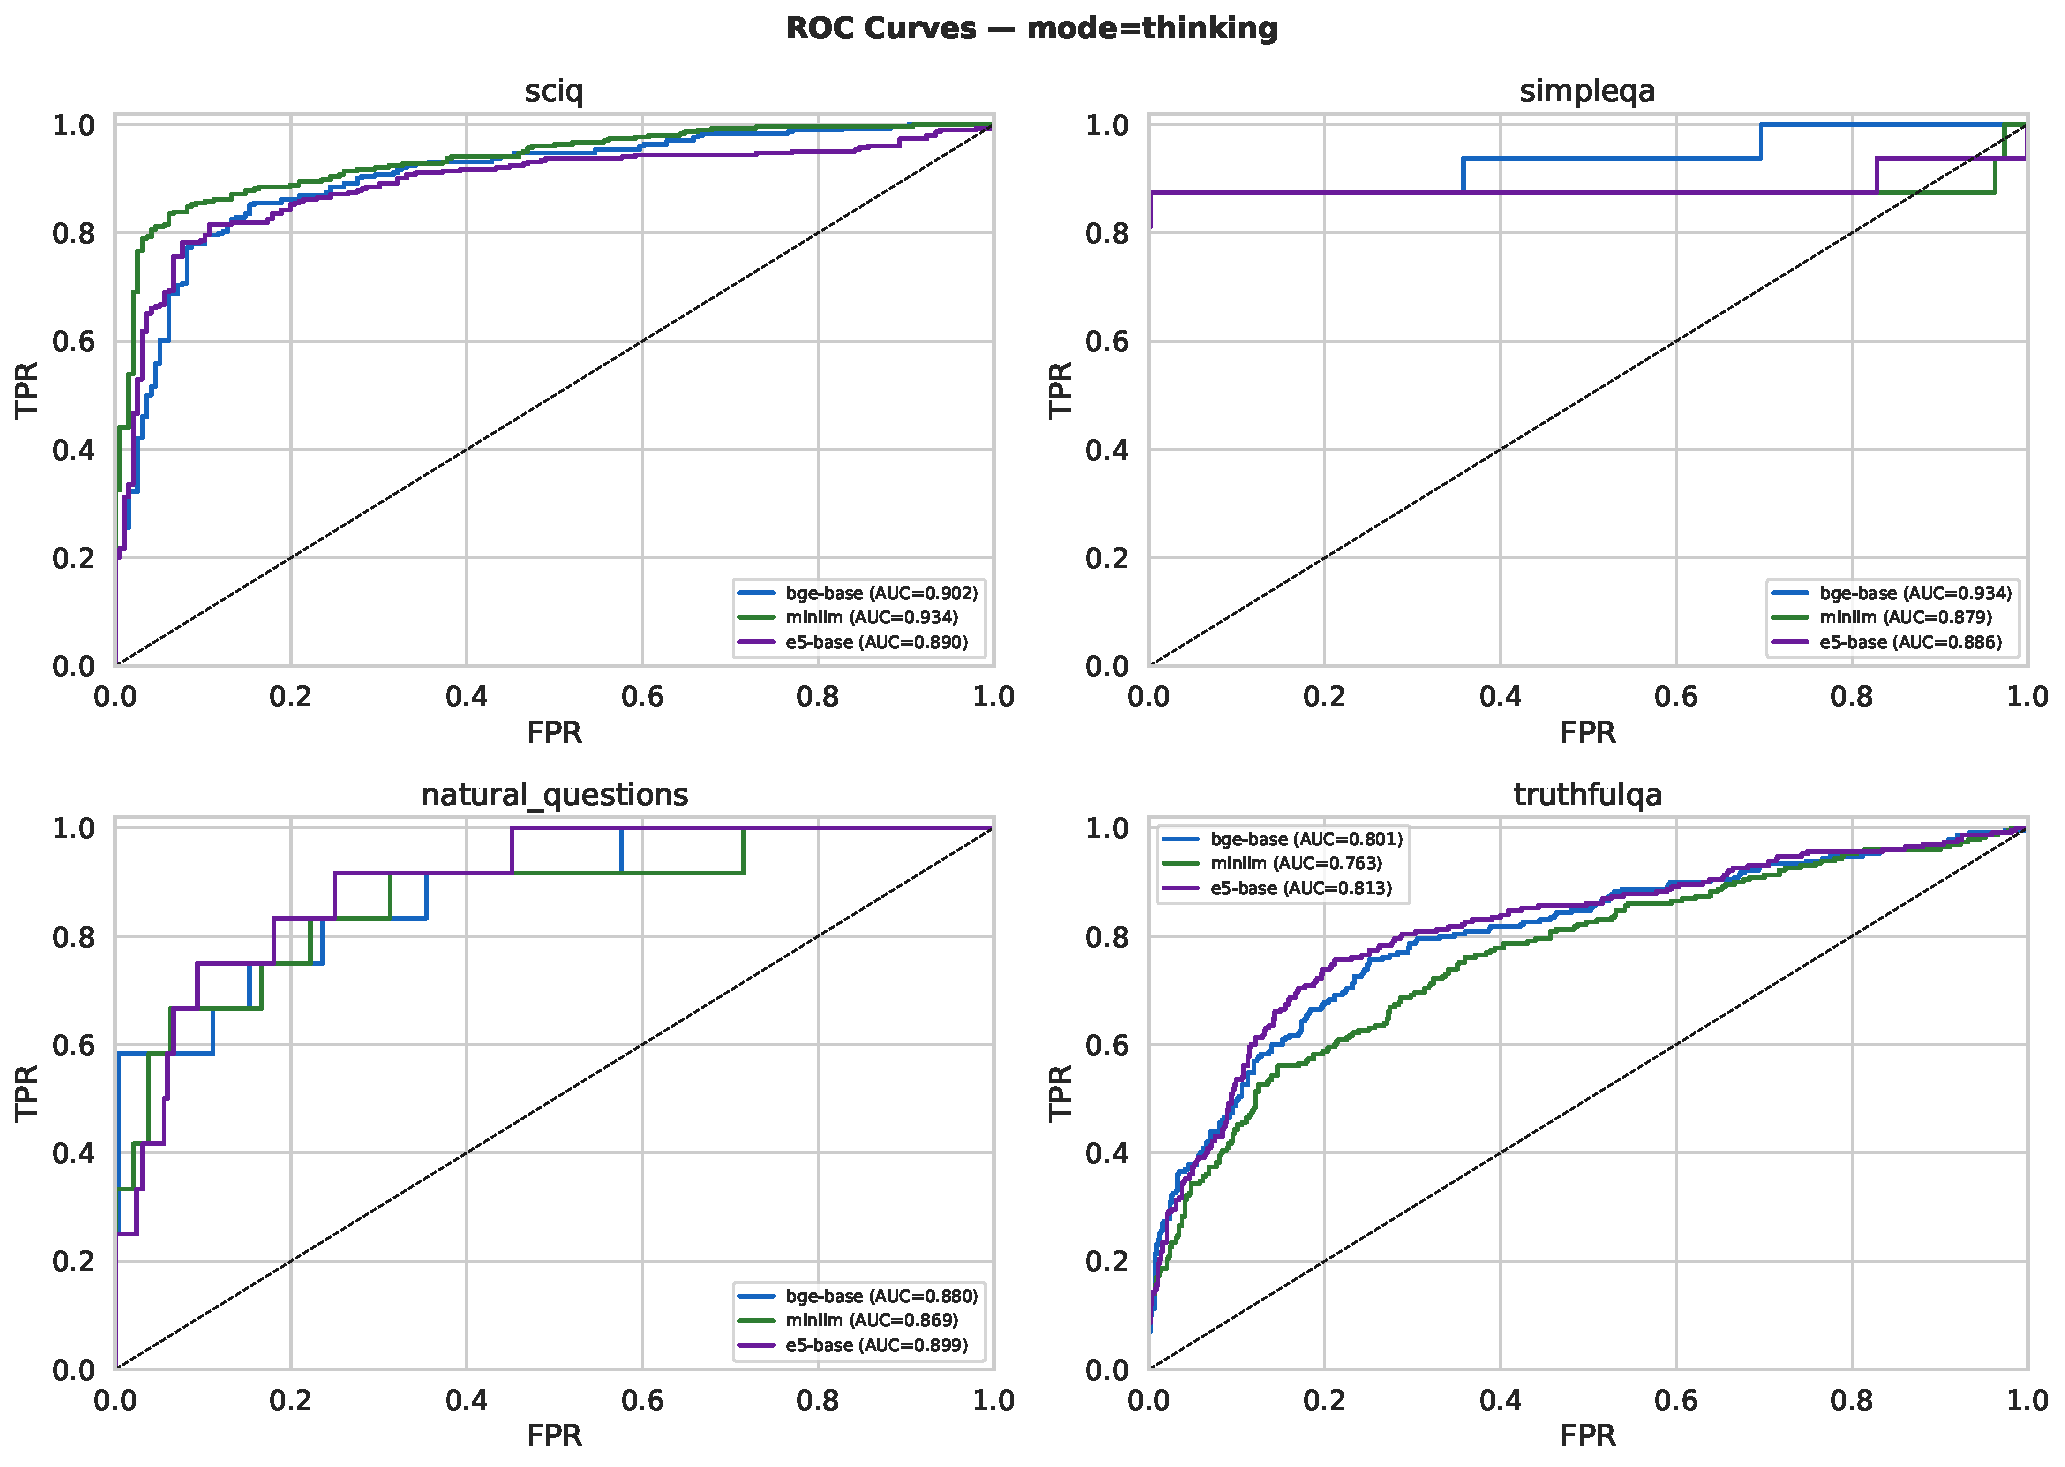
\includegraphics[width=\linewidth]{figures/roc_thinking.pdf}
    \caption{ROC curves --- thinking mode}
  \end{subfigure}
  \caption{ROC curves (BGE-base) for all four datasets.
  Short-form datasets (blue/orange) consistently exhibit higher AUC than
  long-form datasets (green/red).}
  \label{fig:roc}
\end{figure}

\subsection{Short-form vs.\ Long-form QA}
\label{sec:shortlong}

% \Cref{fig:shortlong} visualises the similarity score distributions.
\Cref{fig:shortlong} visualises the short-form vs.\ long-form AUC gap, while \Cref{fig:dist} shows the underlying correct-vs.-incorrect similarity distributions.
The gap between correct and incorrect distributions is substantially wider for
short-form tasks (SciQ $\Delta\bar{s}=0.228$, SimpleQA $\Delta\bar{s}=0.371$)
compared to long-form tasks (NQ $\Delta\bar{s}=0.226$, TruthfulQA $\Delta\bar{s}=0.113$).

The primary reason is \emph{embedding dilution}: long predictions contain background
context, hedge phrases, and irrelevant facts that shift the embedding away from the
core answer vector.
For TruthfulQA, many incorrect predictions are \emph{near-correct paraphrases} of
common misconceptions, whose surface similarity to ground-truth strings is deceptively
high (mean FP similarity 0.865 under BGE).

\begin{figure}[t]
  \centering
  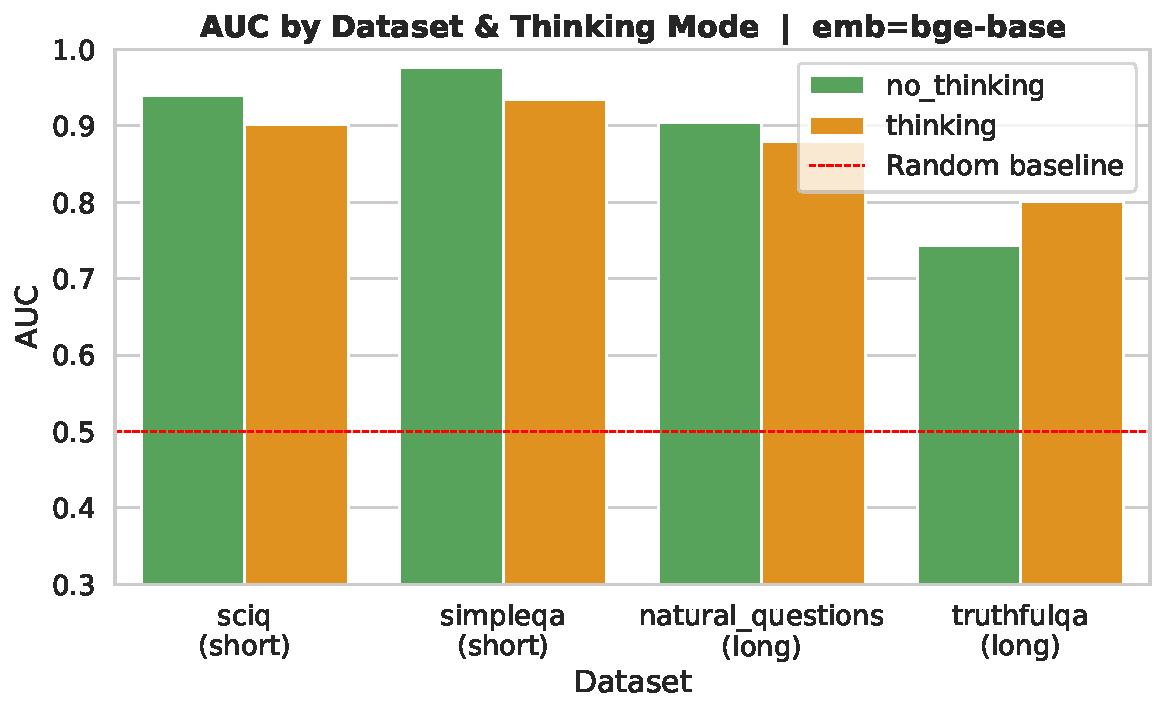
\includegraphics[width=0.7\textwidth]{figures/short_vs_long_bge-base.pdf}
  \caption{AUC comparison: short-form vs.\ long-form QA tasks (BGE-base, no\_thinking).
  The gap confirms the task-type dependence of embedding-based correctness evaluation.}
  \label{fig:shortlong}
\end{figure}

\subsection{Embedding Model Comparison}

\Cref{fig:heatmap} shows AUC heat-maps across all configurations.
MiniLM achieves the highest AUC on SciQ (0.954) but is the weakest on TruthfulQA
(0.723), indicating a strong short-form bias.
BGE performs best on SimpleQA (0.976) and is well-balanced overall.
E5 exhibits the most consistent performance across both short- and long-form tasks,
making it the recommended single-model choice.

\begin{figure}[t]
  \centering
  \begin{subfigure}[b]{0.48\textwidth}
    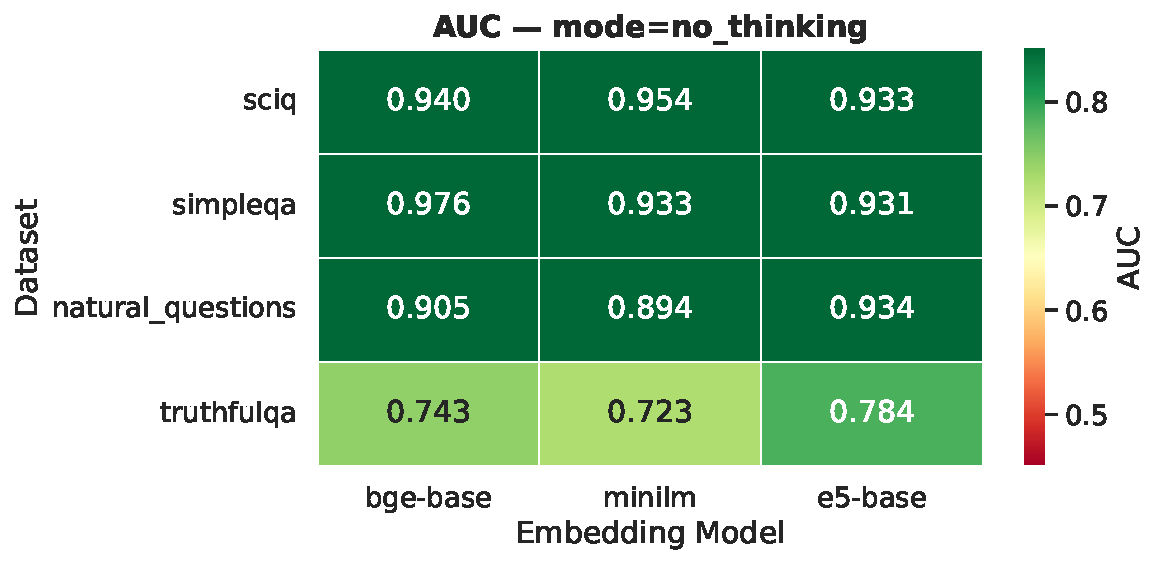
\includegraphics[width=\linewidth]{figures/auc_heatmap_no_thinking.pdf}
    \caption{no\_thinking mode}
  \end{subfigure}\hfill
  \begin{subfigure}[b]{0.48\textwidth}
    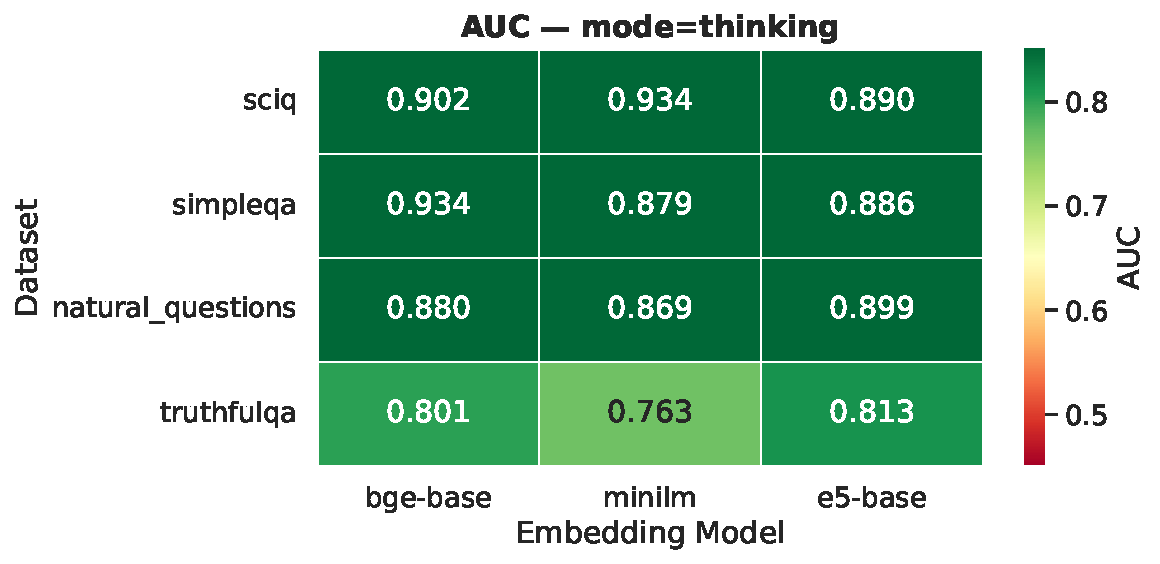
\includegraphics[width=\linewidth]{figures/auc_heatmap_thinking.pdf}
    \caption{thinking mode}
  \end{subfigure}
  \caption{AUC heat-maps (all embedding models and datasets).
  Lighter colour = higher AUC.}
  \label{fig:heatmap}
\end{figure}

\subsection{Ablation: Chain-of-Thought Reasoning Mode}
\label{sec:ablation}

\Cref{fig:ablation} shows the AUC difference between \texttt{thinking} and
\texttt{no\_thinking} modes.
The results reveal a \textbf{bidirectional effect}:

\begin{itemize}[nosep]
  \item \emph{Short-form tasks} (SciQ, SimpleQA): AUC \textbf{decreases} by
        approximately 3--4 points.  CoT responses are longer and embed as denser
        semantic mixtures, increasing the distance from short ground-truth strings.
  \item \emph{TruthfulQA}: AUC \textbf{increases} by 2--3 points.
        CoT reasoning suppresses Qwen3-4B's tendency to echo memorised
        misconceptions; the resulting predictions have clearer separation from
        incorrect alternatives in embedding space
        (BGE mean gap increases from 0.113 to 0.130).
  \item \emph{NQ}: accuracy \emph{drops} from 9.3\% to 4.0\% under thinking mode,
        suggesting that 4B-scale CoT can over-think simple single-hop questions.
\end{itemize}

\begin{figure}[t]
  \centering
  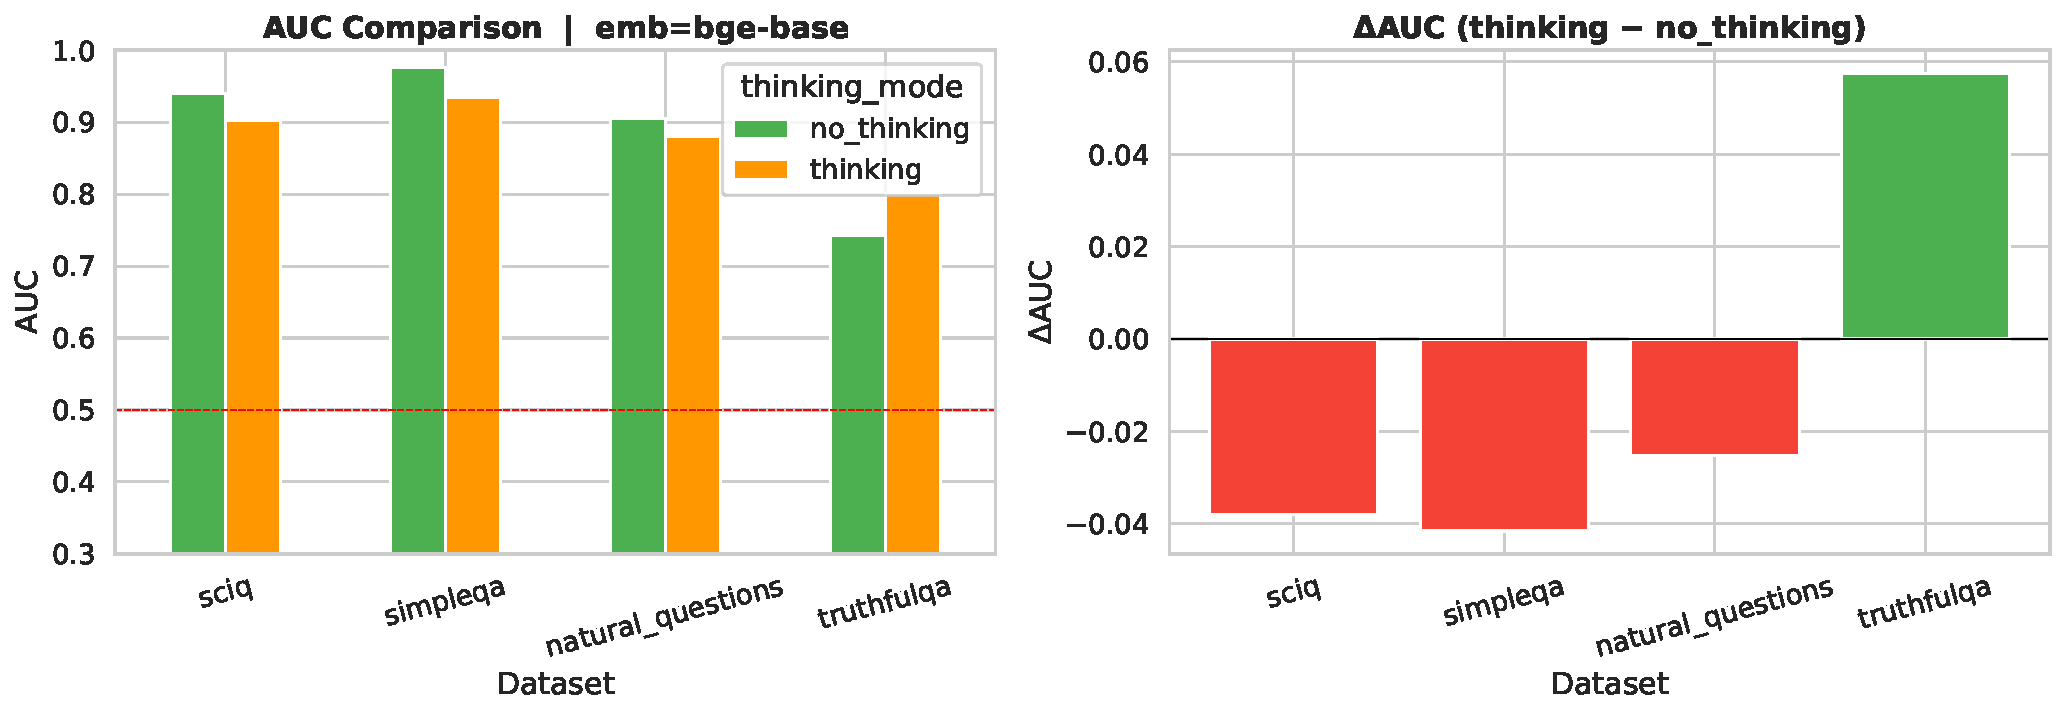
\includegraphics[width=0.65\textwidth]{figures/thinking_ablation_bge-base.pdf}
  \caption{$\Delta$AUC (\texttt{thinking} $-$ \texttt{no\_thinking}) for BGE-base.
  CoT hurts short-form discriminability but slightly helps TruthfulQA.}
  \label{fig:ablation}
\end{figure}

\begin{figure}[t]
  \centering
  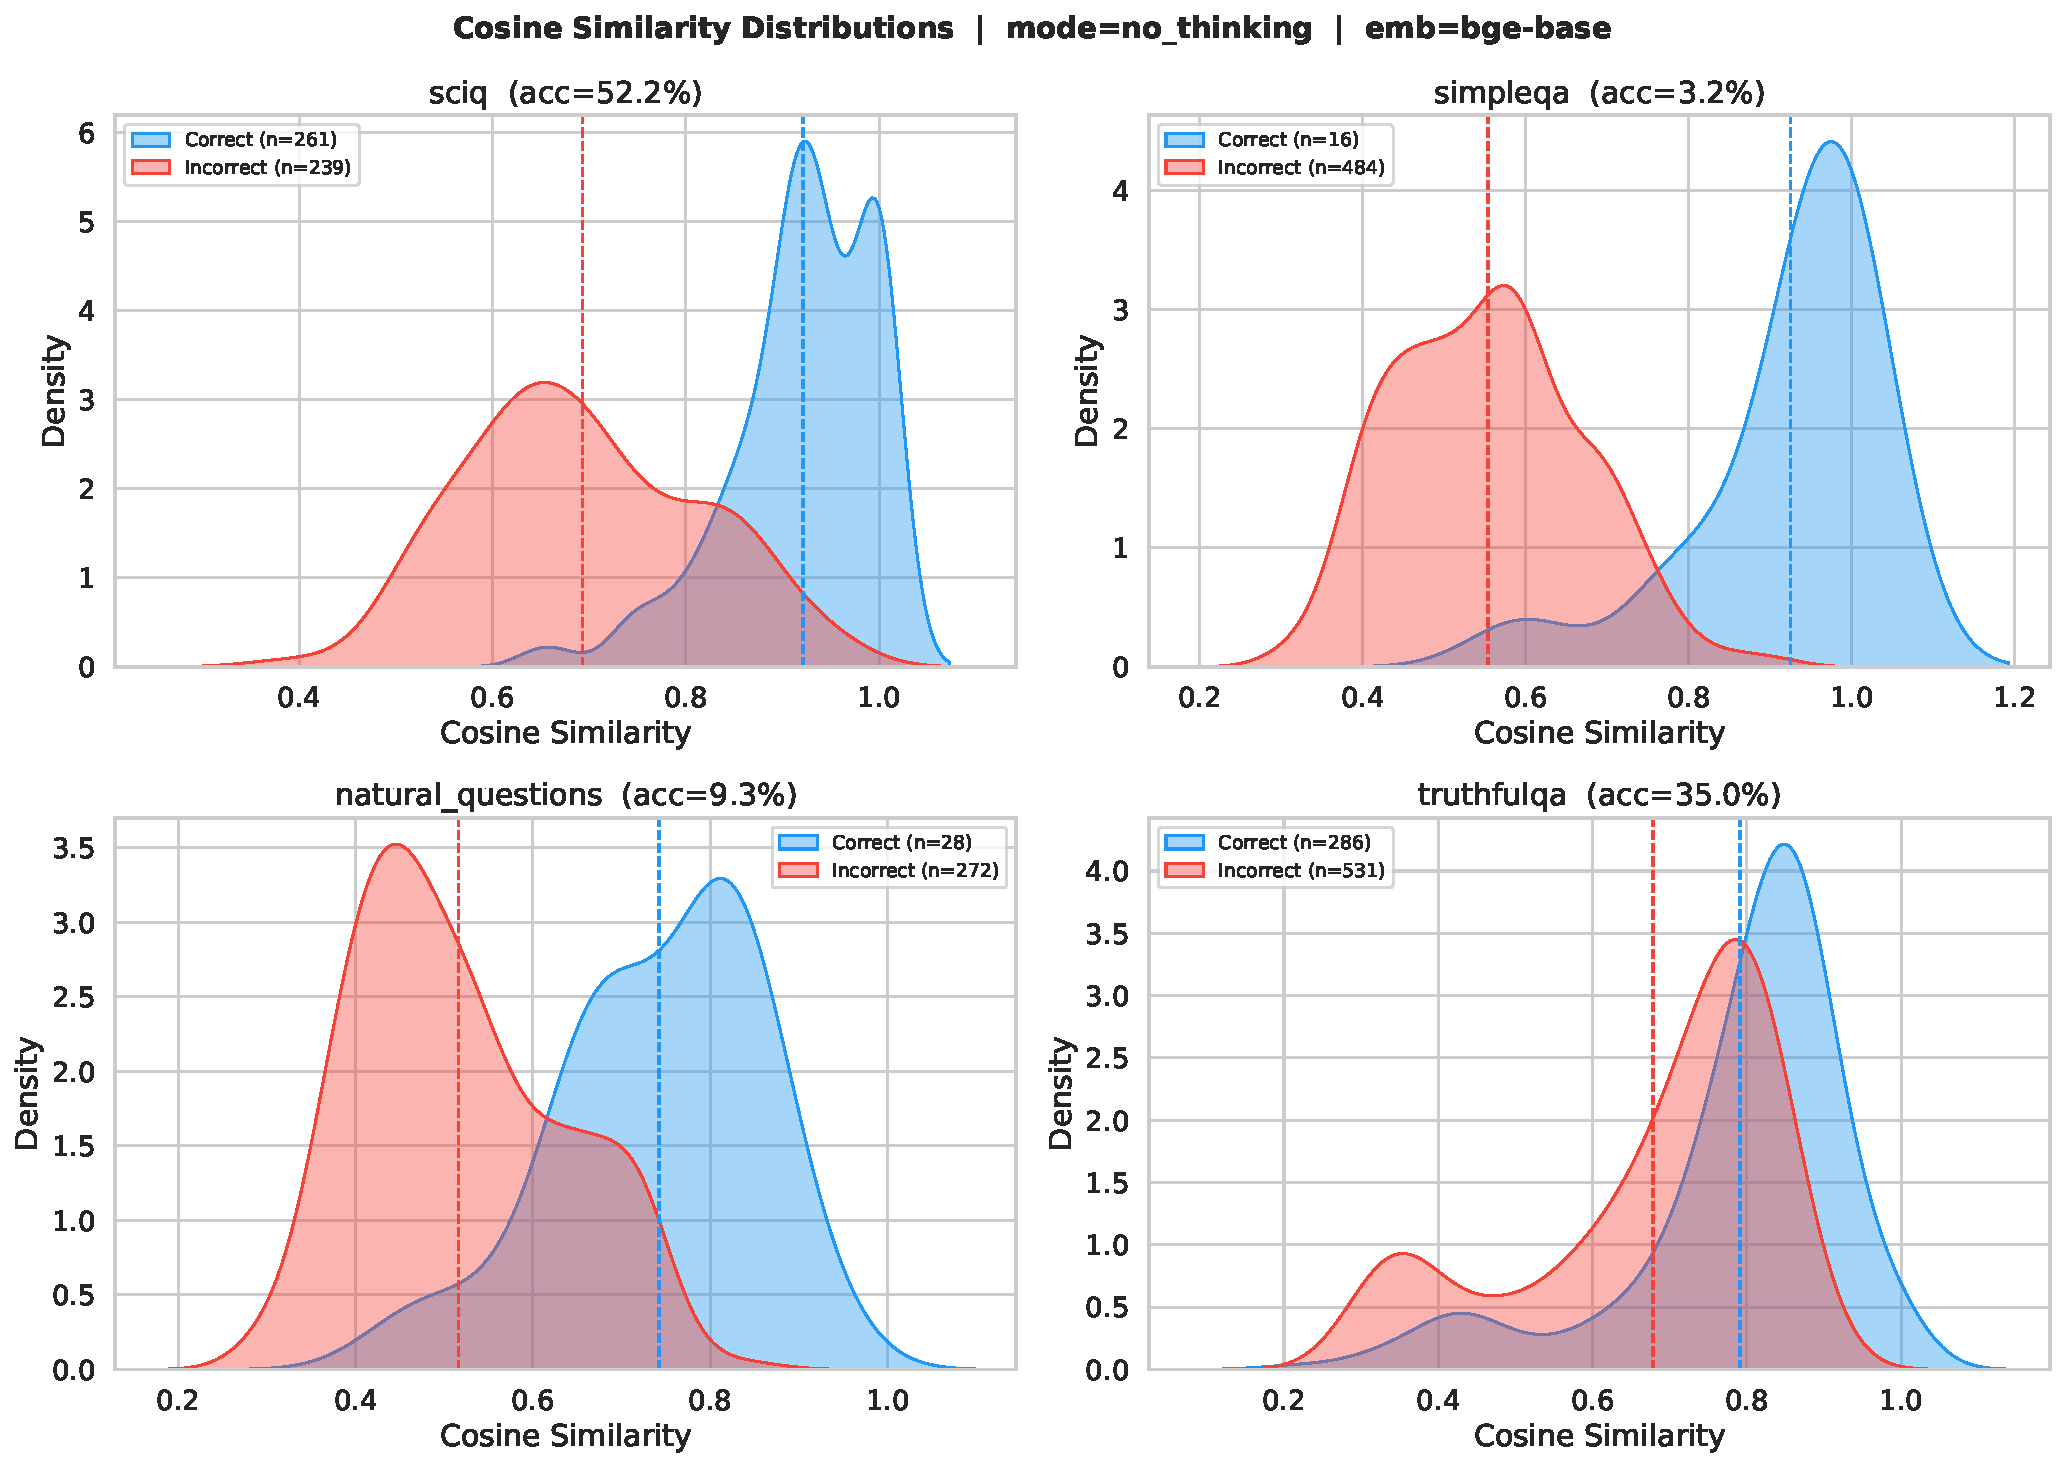
\includegraphics[width=0.72\textwidth]{figures/distributions_no_thinking_bge-base.pdf}
  \caption{Cosine similarity distributions (correct vs.\ incorrect) per dataset,
  BGE-base, no\_thinking mode.  The distribution gap narrows from SimpleQA to
  TruthfulQA, illustrating the short-to-long degradation.}
  \label{fig:dist}
\end{figure}

\subsection{TA Baseline Compatibility Experiments}
\label{sec:ta-baseline}

We additionally evaluate the artifacts produced by
\texttt{scripts/evaluate\_ta\_baseline\_compatibility.py} and by the original TA
pipeline script \texttt{NLI Project v2/run\_all\_datasets.sh}.  The compact
summary is generated by \texttt{scripts/analyze\_added\_experiments.py} under
\texttt{results/added\_experiments/}.

\paragraph{Compatibility predictions.}
The NLP compatibility script has completed no-thinking generation for the two
short-form TA datasets.  On the full TA-prepared splits, the same normalised
exact/contains rule gives the results in \Cref{tab:ta-compat}.

\begin{table}[t]
\centering
\caption{Full-size TA compatibility predictions evaluated with exact/contains matching.}
\label{tab:ta-compat}
\setlength{\tabcolsep}{5pt}
\begin{tabular}{lrrrrr}
\toprule
\textbf{Dataset} & $n$ & \textbf{Exact} & \textbf{Contains/Correct}
  & \textbf{Mean words} & \textbf{Max words} \\
\midrule
SciQ                & 13,679 & 41.3\% & \textbf{55.8\%} & 1.89 & 196 \\
SimpleQuestionsWiki & 49,202 & 12.1\% & \textbf{16.6\%} & 2.83 & 222 \\
\bottomrule
\end{tabular}
\end{table}

The pattern is consistent with the main benchmark: SciQ is substantially easier
than SimpleQuestions-style factual recall under strict lexical matching.  The long
maximum prediction lengths also show that a small number of nominally short-form
generations violate the requested format, which can distort embedding similarity
unless filtered or span-normalised.

\paragraph{Original TA pipeline artifacts.}
After fixing the HHEM tied-weight loading bug and rerunning
\texttt{EVAL\_DEVICE=cuda:0 ./rerun\_hhem\_fixed.sh sciq truthfulQA}, the
original TA artifacts provide valid HHEM and MPNet outputs for SciQ and
TruthfulQA, while NQ currently has predictions only (\Cref{tab:ta-original}).

\begin{table}[t]
\centering
\caption{Summary of original TA pipeline artifacts. HHEM is thresholded at 0.5.}
\label{tab:ta-original}
\small
\setlength{\tabcolsep}{4pt}
\begin{tabular}{lrrrrrrr}
\toprule
\textbf{Dataset} & \textbf{Pred.} & \textbf{HHEM n} & \textbf{HHEM mean}
  & \textbf{HHEM+} & \textbf{Unique} & \textbf{MPNet mean} & \textbf{MPNet med.} \\
\midrule
SciQ       & 13,679 & 13,679 & 0.2874 & 25.9\% & 13,357 & 0.762 & 0.794 \\
TruthfulQA &    817 &    817 & 0.1466 & 10.4\% &    817 & 0.560 & 0.545 \\
NQ         &  3,400 &      0 & --     & --      & 0 & --    & --    \\
\bottomrule
\end{tabular}
\end{table}

Corrected HHEM is now discriminative and much stricter than exact/contains
matching.  SciQ has a higher HHEM positive rate than TruthfulQA (25.9\% vs.\
10.4\%), and its merged-statement MPNet similarity is also higher (0.762 vs.\
0.560 mean cosine).  Using HHEM $\ge 0.5$ as the label, MPNet cosine reaches
AUC 0.712 on SciQ and 0.659 on TruthfulQA.  The corrected TA pipeline therefore
supports the short-form/long-form degradation observed in \Cref{sec:shortlong}.

% ── 6. Failure Analysis ───────────────────────────────────────────────────────
\section{Failure Analysis}
\label{sec:failure}

We extract the top-50 false positives (FP: high similarity but incorrect) and
top-50 false negatives (FN: low similarity but correct) per configuration using
the Youden-optimal threshold, and categorize them using rule-based diagnostic
heuristics.
We then inspect representative cases from each category to interpret the dominant
error patterns.
The failure categories should be understood as diagnostic labels rather than
human-annotated ground truth.

\paragraph{Lexical variation.}
The prediction contains the correct factual content but uses different surface forms
(synonyms, abbreviations, paraphrases).
Example: prediction ``H\textsubscript{2}O'' vs.\ ground truth ``water''.
Affects primarily short-form tasks (SciQ: 14 FP/FN; SimpleQA: 22 FP/FN).

\paragraph{Semantic ambiguity.}
The question admits multiple plausible answers that occupy overlapping regions of
embedding space, making threshold-based separation unreliable.
Example: TruthfulQA Q: ``What is the most popular sport in America?''---both
``American football'' and ``baseball'' achieve high similarity to the ground truth
string ``American football''.
Affects SciQ (16 cases) and SimpleQA (11 cases).

\paragraph{Long-form reasoning complexity.}
The prediction embeds as a mixture of correct and incorrect content, or correctly
cites a misconception while refuting it (e.g., ``Fortune cookies did not originate
in China; they were invented in Japan/USA''), inflating cosine similarity with the
wrong-answer ground truth.
This is the dominant failure type for NQ and TruthfulQA (51 and 100+ cases
respectively, \Cref{fig:failure}).

\begin{figure}[t]
  \centering
  \begin{subfigure}[b]{0.48\textwidth}
    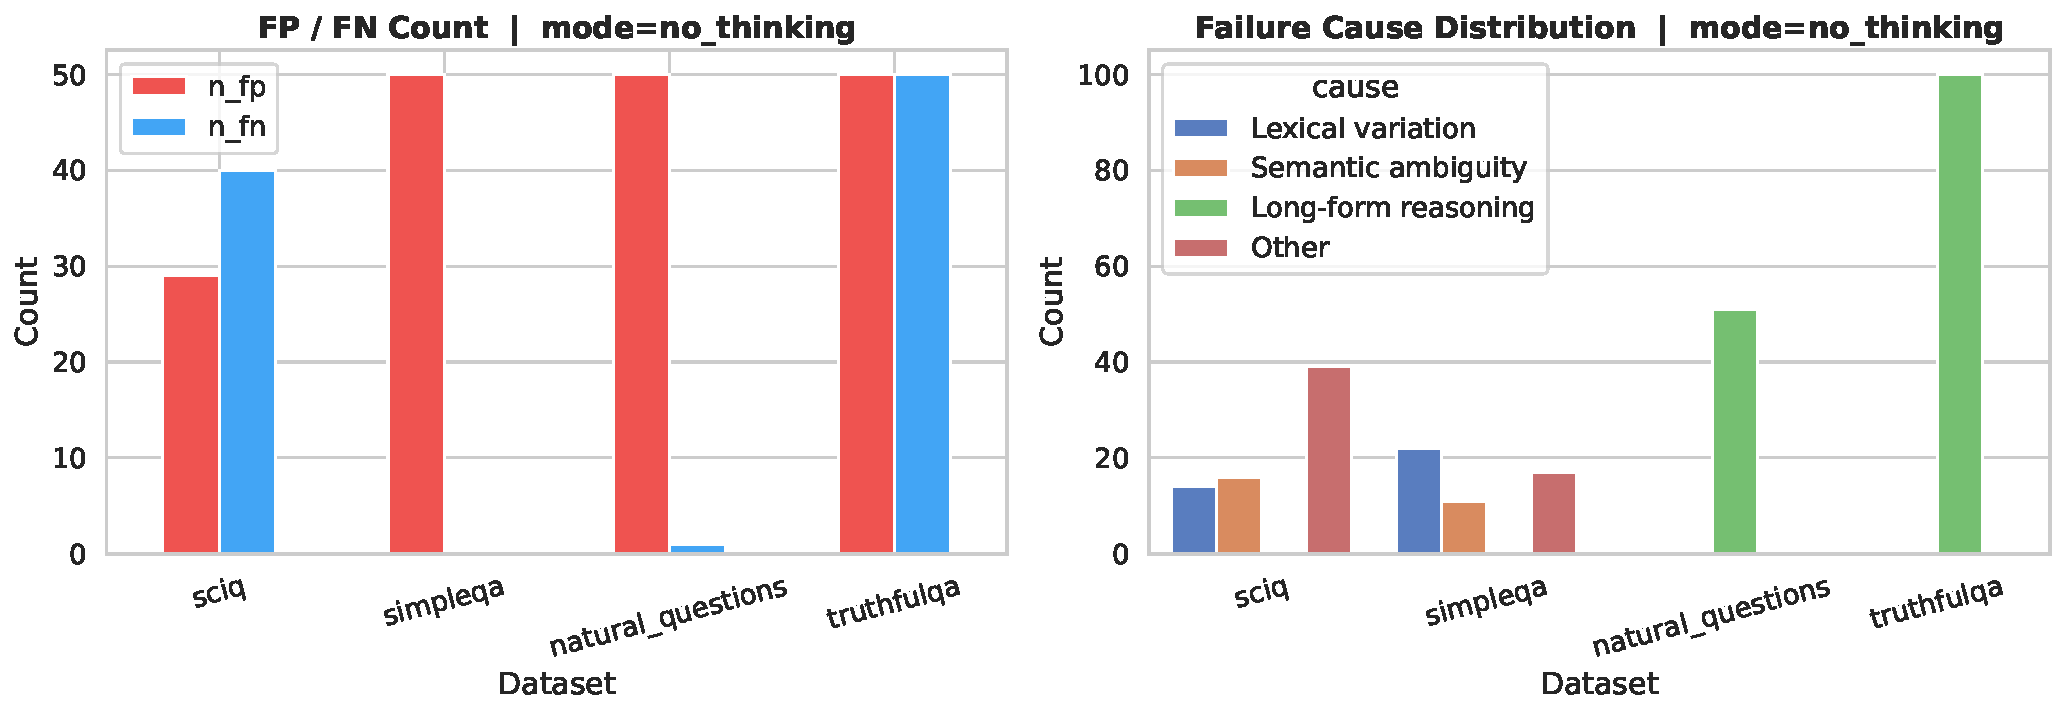
\includegraphics[width=\linewidth]{figures/failure_causes_no_thinking.pdf}
    \caption{no\_thinking mode}
  \end{subfigure}\hfill
  \begin{subfigure}[b]{0.48\textwidth}
    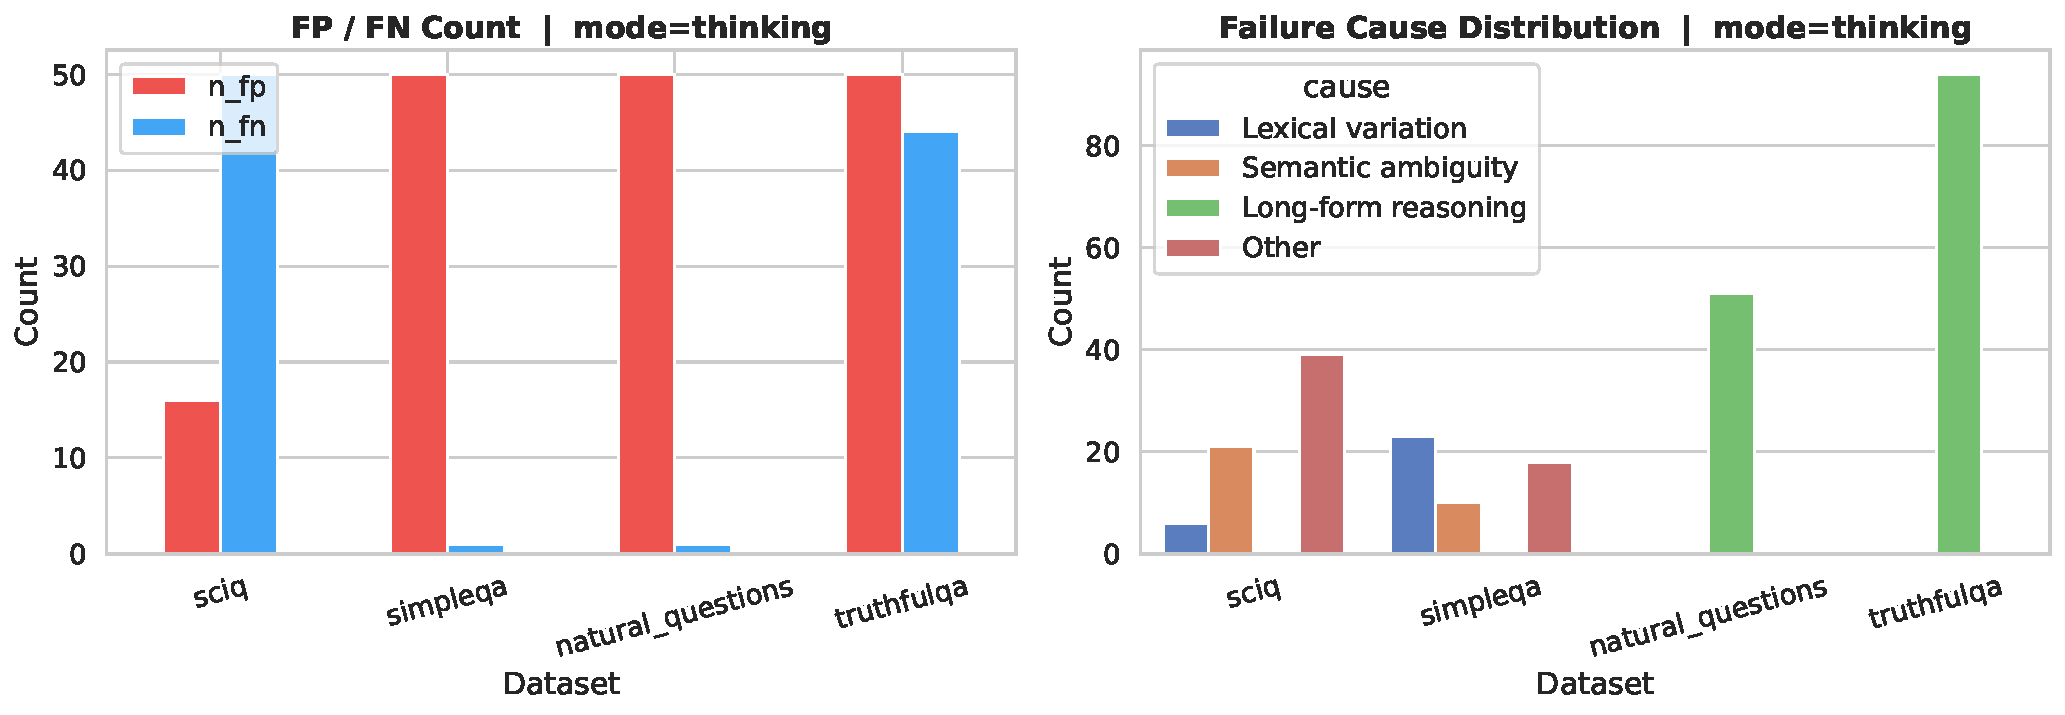
\includegraphics[width=\linewidth]{figures/failure_causes_thinking.pdf}
    \caption{thinking mode}
  \end{subfigure}
  \caption{Failure cause distribution across datasets and generation modes.
  Long-form reasoning complexity dominates NQ and TruthfulQA errors.}
  \label{fig:failure}
\end{figure}

\paragraph{Format mismatch (CoT-specific).}
When the ground truth is an ultra-short string (e.g., ``2002'') and the prediction
is a full sentence (``\emph{Catch Me If You Can} was made in 2002''), the
\emph{contains-match} criterion correctly labels it as correct, but the embedding
of the full sentence is far from that of ``2002'' in cosine space.
This systematic bias explains a significant fraction of the AUC drop from
\texttt{no\_thinking} to \texttt{thinking} on SimpleQA.

\Cref{tab:failure} summarises the failure statistics.

\begin{table}[t]
\centering
\caption{Failure counts (top-50 FP + FN) per dataset (BGE-base, no\_thinking).}
\label{tab:failure}
\setlength{\tabcolsep}{5pt}
\begin{tabular}{lrrrrr}
\toprule
\textbf{Dataset} & \textbf{FP} & \textbf{FN}
  & \textbf{Lexical} & \textbf{Ambiguity} & \textbf{Long-form} \\
\midrule
SciQ       & 29 & 40 & 14 & 16 &  0 \\
SimpleQA   & 50 &  0 & 22 & 11 &  0 \\
NQ         & 50 &  1 &  0 &  0 & 51 \\
TruthfulQA & 50 & 50 &  0 &  0 & 100 \\
\bottomrule
\end{tabular}
\end{table}

\paragraph{Heuristic label caveat.}
The failure-cause labels are produced by task-type rules; in particular,
long-form QA cases are assigned to the long-form reasoning category by task type,
so the counts should be interpreted as qualitative diagnostics rather than precise
human annotations.

% ── 7. Improvement Methods ────────────────────────────────────────────────────
\section{Improvement Methods and Results}
\label{sec:improvement}

Motivated by the failure analysis, we propose and evaluate four strategies.

\subsection{Method A: Post-hoc Poincaré Projection}

We apply the exponential map to project Euclidean embeddings onto the Poincaré ball:
\begin{equation}
  \mathbf{y} = \text{expmap}_0(\alpha \mathbf{x}), \quad \alpha = 0.05
\end{equation}
followed by the Poincaré distance as a replacement for cosine distance.
\textbf{Result: $\Delta$AUC $\approx$ 0} across all 24 configurations.
The reason is that AUC is a rank-invariant metric: a monotone bijection from
Euclidean to hyperbolic distance cannot change the ranking of pairs and therefore
cannot change AUC.
This is an important negative result confirming that post-hoc geometric
re-projection is insufficient; hyperbolic gains require training in hyperbolic space
from the start.

\subsection{Method B: Sentence-level MaxSim}

Instead of comparing document-level embeddings, we split the prediction into
sentences, encode each sentence independently, and compute:
\begin{equation}
  s_{\text{MaxSim}} = \max_{j} \cos(\mathbf{e}_{p_j}, \mathbf{e}_g)
\end{equation}
\textbf{Results} (\Cref{tab:improvement}):
MaxSim consistently helps in the \texttt{thinking} mode for SciQ and SimpleQA
(e.g., BGE $\Delta$AUC = $+$0.047 on SimpleQA/thinking) by isolating the final
answer sentence from CoT verbosity.
However, it \emph{harms} performance on NQ and TruthfulQA ($\Delta$AUC up to
$-$0.087) because long-form predictions often contain sentences that mention
ground-truth entities in a refutational context, generating false-positive matches.

\subsection{Method C: HELM Trained Hyperbolic Projection}

Inspired by \citet{he2025helm}, we train a lightweight MLP projection head
($\text{Linear}(D, 256) \to \text{ReLU} \to \text{Linear}(256, 256)$) that maps
Euclidean embeddings into the Poincaré ball.
Training uses binary cross-entropy on correct/incorrect pairs with a
RiemannianAdam optimiser over 30 epochs, with 80/20 train/test splits.
Validation AUCs: BGE 0.934, MiniLM 0.937, E5 \textbf{0.952}.
Since HELM is evaluated only on the held-out test split, its numbers are not
directly comparable to full-set post-hoc methods unless the baseline is recomputed
on the same split.

\textbf{Results (held-out test split)}: HELM provides the largest and most
consistent gains on TruthfulQA (BGE $+$9.9, MiniLM $\approx$$+$8.0,
E5 $\approx$$+$5.8 AUC points), demonstrating that hierarchical hyperbolic geometry
captures the \emph{contrastive} semantic structure of adversarial answers better than
Euclidean cosine similarity.
Gains on SciQ and SimpleQA/no\_thinking are moderate (+1--+6 AUC points).
NQ/thinking results are noisy due to the small test set ($n_{\text{pos}}=4$).

\subsection{Method D: Span-MaxSim}

We identify ``answer indicator'' spans in CoT predictions using regex patterns
(\emph{``the answer is'', ``therefore'', ``thus''}, etc.) and embed only the
extracted final-answer sentence.
\textbf{Results}: Span-MaxSim provides small positive gains on NQ/thinking
($\Delta$AUC $+$0.7--$+$1.6 AUC points) but hurts TruthfulQA/thinking
significantly ($-$8.2 to $-$9.3 AUC points) because multi-answer ground truths
require full-prediction coverage for accurate MaxSim, which span extraction destroys.

\begin{table}[t]
\centering
\caption{$\Delta$AUC relative to baseline for all improvement methods
(BGE-base).  Poincaré, MaxSim, and Span-MaxSim are evaluated on the full set;
HELM is evaluated on its held-out test split only.  Best per row in \textbf{bold}.}
\label{tab:improvement}
\setlength{\tabcolsep}{4.5pt}
\begin{tabular}{llrrrr}
\toprule
\textbf{Dataset} & \textbf{Mode}
  & \textbf{Poincaré} & \textbf{MaxSim} & \textbf{HELM} & \textbf{Span-MaxSim} \\
\midrule
SciQ       & no\_thinking & 0.000 & $\approx$0  & \textbf{+0.012} & $\approx$0 \\
SciQ       & thinking     & 0.000 & +0.017 & \textbf{+0.057} & +0.005 \\
SimpleQA   & no\_thinking & 0.000 & $\approx$0  & \textbf{+0.038} & $\approx$0 \\
SimpleQA   & thinking     & 0.000 & \textbf{+0.047} & $\approx$0  & $\approx$0 \\
NQ         & no\_thinking & 0.000 & $-$0.023 & \textbf{+0.032} & $\approx$0 \\
NQ         & thinking     & 0.000 & $-$0.036 & \textbf{+0.045} & +0.016 \\
TruthfulQA & no\_thinking & 0.000 & $-$0.036 & \textbf{+0.052} & 0.000 \\
TruthfulQA & thinking     & 0.000 & $-$0.057 & \textbf{+0.098} & $-$0.093 \\
\bottomrule
\end{tabular}
\end{table}

\begin{figure}[t]
  \centering
  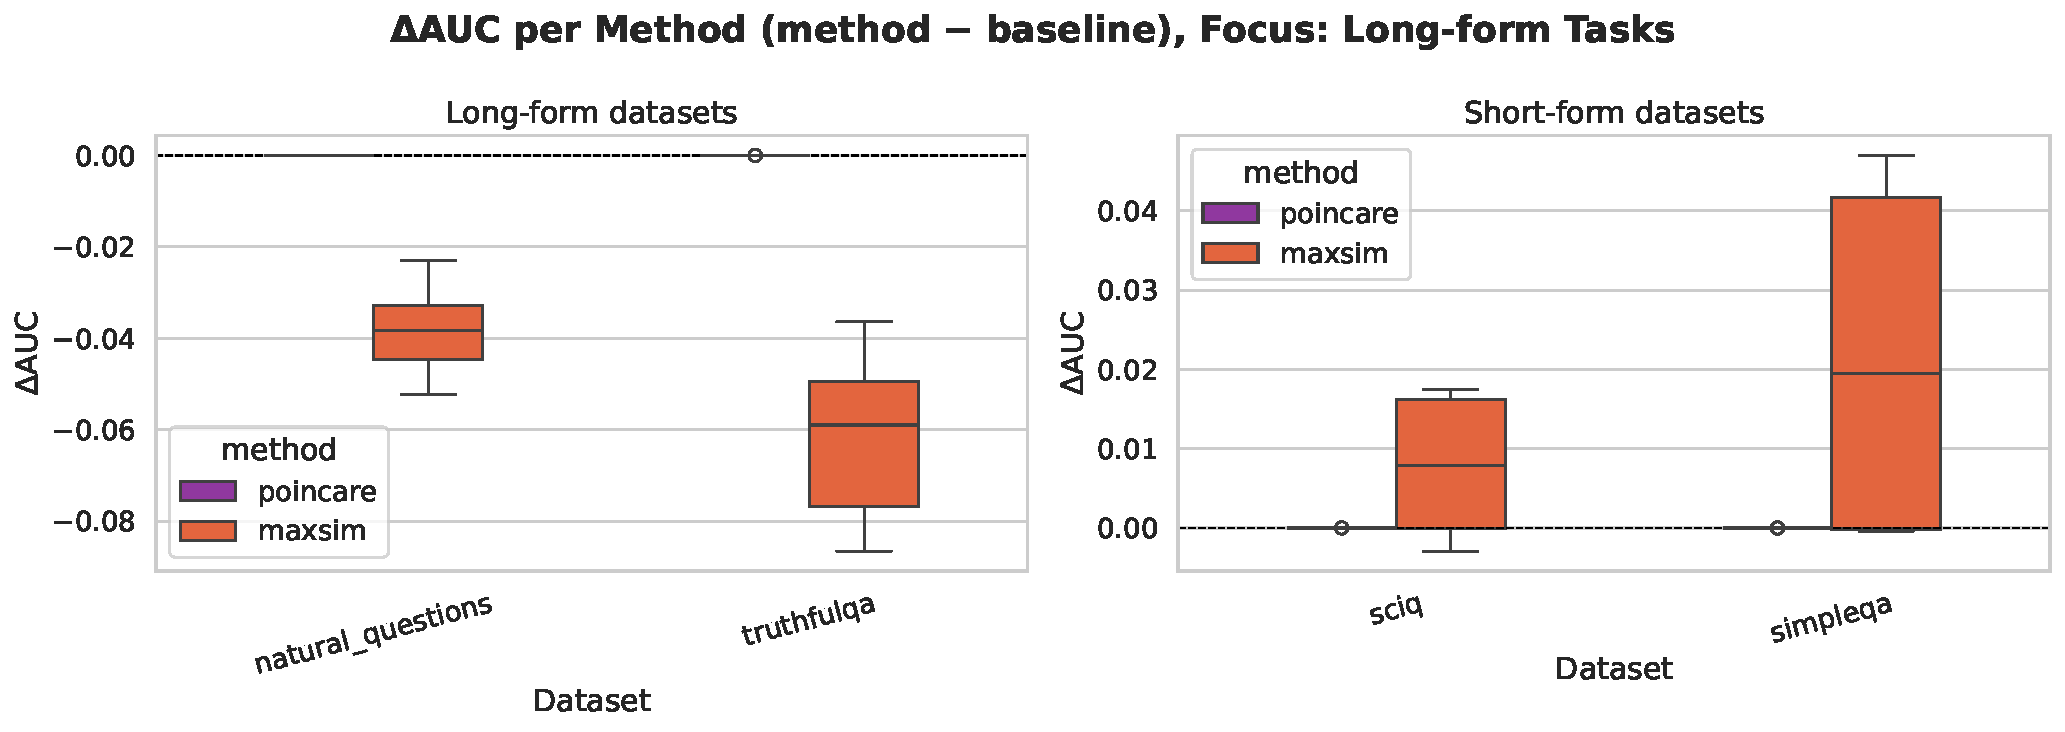
\includegraphics[width=0.72\textwidth]{figures/delta_auc_boxplot.pdf}
  \caption{$\Delta$AUC distribution for each improvement method across all 24
  configurations.  HELM is consistently positive; MaxSim is bimodal;
  Poincaré is uniformly zero; Span-MaxSim has a long negative tail.}
  \label{fig:delta}
\end{figure}

\paragraph{Summary.}
The results highlight a fundamental dichotomy: \emph{structural} improvements
(trained hyperbolic projection) yield consistent cross-task gains, while
\emph{heuristic} improvements (MaxSim, Span extraction) are task- and mode-specific.
For production use, HELM-style training is the recommended approach for long-form QA
evaluation; MaxSim is a useful add-on for CoT-based short-form tasks.

% ── 8. Limitations ────────────────────────────────────────────────────────────
\section{Limitations}
\label{sec:limitations}

\begin{enumerate}[nosep]
  \item \textbf{Silver correctness labels.}  Correctness labels are produced by
        automatic rules (exact match, token-F1, or accepted-answer lists) rather
        than human annotations.  Tasks requiring subjective judgement may need
        human-validated labels.
  \item \textbf{Single ground-truth reference.}  The embedding similarity is
        computed against the first ground-truth string.  For datasets with multiple
        valid paraphrase answers, this may underestimate semantic equivalence.
  \item \textbf{Class imbalance.}  Some datasets are heavily imbalanced---SimpleQA
        has a correctness rate of only 3.2\%---which can inflate AUC variance for
        small positive sets.
  \item \textbf{HELM test-split evaluation.}  The trained hyperbolic projection is
        evaluated on a held-out split rather than the full dataset.  Direct numerical
        comparison with full-set post-hoc methods should be interpreted carefully.
\end{enumerate}

% ── 9. Conclusion ─────────────────────────────────────────────────────────────
\section{Conclusion}
\label{sec:conclusion}

We systematically investigated whether cosine similarity in embedding space is a
reliable proxy for LLM prediction correctness across four QA benchmarks.
Our study yields five key takeaways:

\begin{enumerate}[nosep]
  \item \textbf{Short-form QA: yes, reliably.}  AUC reaches 0.976 (SimpleQA/BGE),
        and all similarity distributions are highly separated ($p < 10^{-8}$).
  \item \textbf{Long-form QA: only partially.}  TruthfulQA AUC peaks at 0.813,
        reflecting the inability of Euclidean cosine to separate contrastive
        adversarial answers.
  \item \textbf{CoT reasoning has opposing effects.}  It hurts short-form
        discriminability (format mismatch) but helps TruthfulQA (suppresses
        hallucination echoes).
  \item \textbf{Trained hyperbolic projection is the most effective improvement.}
        HELM provides consistent +0.052--+0.098 AUC point gains on TruthfulQA
        (held-out test split) without dataset-specific engineering.
  \item \textbf{TA baseline compatibility is partially validated.}  The
        compatibility script processes full-size TA SciQ and SimpleQuestionsWiki
        predictions, and corrected TA HHEM/MPNet outputs reproduce the
        short-vs-long degradation: SciQ has higher HHEM consistency (25.9\%)
        and MPNet cosine (0.762) than TruthfulQA (10.4\%, 0.560).
\end{enumerate}

Future work should investigate training HELM jointly with the LLM fine-tuning
objective, and extending the framework to RAG settings where faithfulness and
factual correctness must both be evaluated simultaneously.

\section*{Contributions of Individual Members}

All group members contributed to this project. The main responsibilities were:

\begin{itemize}[nosep]
  \item Haodong Xu: Completed the main coding work and experiments, and drafted part of the report.
  \item Chi Kit WONG: Created the poster and the methodology diagram for the Methodology section.
  \item Sida Zhang: Implemented improvement methods and proofread the paper.
\end{itemize}

% ── References ────────────────────────────────────────────────────────────────
\bibliographystyle{unsrtnat}
\bibliography{references}

% ── Appendix ──────────────────────────────────────────────────────────────────
\appendix
\section{Report--Code Mapping}
\label{sec:appendix}

\begin{table}[ht]
\centering
\caption{Mapping from report components to implementation files.}
\label{tab:code-mapping}
\begin{tabular}{p{0.33\linewidth} p{0.53\linewidth}}
\toprule
\textbf{Report component} & \textbf{Implementation source} \\
\midrule
Dataset preparation & \texttt{scripts/prepare\_data.py} \\
Qwen3-4B generation & \texttt{scripts/generate\_predictions.py} \\
Correctness labeling & \texttt{src/evaluation/correctness.py} \\
Embedding extraction & \texttt{scripts/encode\_embeddings.py} \\
AUC / ROC analysis & \texttt{scripts/similarity\_analysis.py}, \texttt{results/summary\_auc.csv} \\
Failure analysis & \texttt{scripts/failure\_analysis.py}, \texttt{results/failure\_summary.csv} \\
Improvement methods & \texttt{scripts/improvement\_analysis.py}, \texttt{scripts/train\_hyperbolic.py} \\
TA baseline compatibility & \texttt{scripts/evaluate\_ta\_baseline\_compatibility.py} \\
\bottomrule
\end{tabular}
\end{table}

\end{document}
